% Created 2021-12-28 Tue 18:39
% Intended LaTeX compiler: xelatex
\documentclass[11pt,twoside,landscape]{article}
\usepackage{graphicx}
\usepackage{longtable}
\usepackage{wrapfig}
\usepackage{rotating}
\usepackage[normalem]{ulem}
\usepackage{amsmath}
\usepackage{amssymb}
\usepackage{capt-of}
\usepackage{hyperref}
\usepackage[newfloat]{minted}
\usepackage{color}
\usepackage{listings}
\usepackage[top=2cm,bottom=2cm,right=2cm,left=2cm,landscape]{geometry}
\usepackage{multicol}
\usepackage{enumitem}
\setlist{noitemsep}
\setlength{\parindent}{0pt}
\setlength{\columnseprule}{0.2pt}
\setcounter{secnumdepth}{0}
\author{Olivier Lischer}
\date{\today}
\title{Experimentieren und Evaluieren}
\hypersetup{
 pdfauthor={Olivier Lischer},
 pdftitle={Experimentieren und Evaluieren},
 pdfkeywords={},
 pdfsubject={},
 pdfcreator={Emacs 27.2 (Org mode 9.5.1)}, 
 pdflang={English}}
\begin{document}

\begin{multicols}{3}
\section*{{\bfseries\sffamily TODO} Versuchsplanung}
\label{sec:org8a1115c}
\subsection*{{\bfseries\sffamily TODO} Grundbegriffe}
\label{sec:org58ed7dd}
\begin{itemize}
\item \textbf{Testverteilung}: Können benutzt werden um Ergebnisse von Experimente miteinander zu vergleichen
\item \textbf{Hypothese}: Eine Annahme
\item \textbf{Zielgrösse}: Ergebnis eines Versuchs
\item \textbf{Einflussgrössen}:
\begin{itemize}
\item \textbf{Störgrössen (Rauschen)}: können nicht eingestellt werden
\item \textbf{Steuergrösse}: können eingestellt und gehalten werden
\end{itemize}
\item \textbf{Faktoren}: für den Verusch wesentlichen Einflussgrössen
\item \textbf{Faktorarten}:
\begin{itemize}
\item \textbf{Quantitativ}: beschreiben Zahlenwerte auf der Messskala
\item \textbf{Qualitativ}: Name, Beschreibung, Bezeichnung
\end{itemize}
\end{itemize}
\subsection*{Wissenserwerbs Shewhart}
\label{sec:org3ce64d2}
\begin{center}
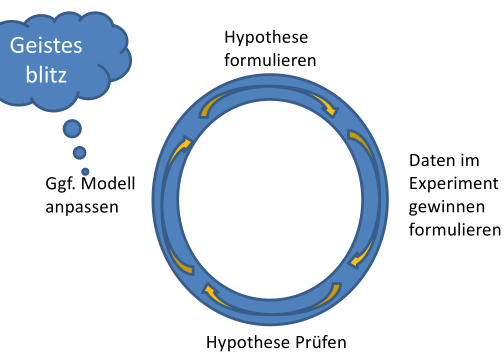
\includegraphics[width=.9\linewidth]{img/shewhart.png}
\end{center}

\subsection*{DoE}
\label{sec:org1c92871}
\begin{enumerate}
\item Ausgangssituation und Problem beschreiben: Problem wirklich verstanden?
\item Untersuchungsziel festlegen: Was wollen wir erreichen?
\item Zielgrössen und Faktoren festlegen
\item Entscheidung: Soll das Problem analytisch / experimentell gelöst werden? Nein => Ende
\item Planung
Versuchplan aufstellen, Blockbildung, Aufwandsabschätzung
\item Entscheidung: Experiment am realen Object oder Model durchführen?
\item Nachbearbeitung
Versuch durchführen, Ergebnisse auswerten, intepretieren und Massnahmen ableiten, Absicherung, Dokumentation und weiteres Vorgehen
\end{enumerate}

\subsection*{Daten sammeln}
\label{sec:org0020847}
Was ist der Anlass, Daten zu sammeln?
\begin{itemize}
\item Reine Sammelwut (Big Data, Data Minig) um im Nachgang Zusammenhänge zu finden
\item bewusstes erfassen von Daten (Data-Farming) um Normen einhalten zu könne, Schwachstellen zu erkennen
\end{itemize}

\subsection*{Statitische Grundbegriffe}
\label{sec:org2707339}
\textbf{Merkmalsträger} (Mensch, Maschine, etc.). \textbf{Grundgesamtheit} ist die Menge aller Merkmalsträger. \textbf{Merkmal} (Augenfarbe, Ausfallrate) sind die Eingeschaften des Merkmalträgers. \textbf{Merkmalswert} (Blaue Auge, 5mal pro Stunde) sind die Ausprägung der Merkmale.
\subsection*{Skalen}
\label{sec:org50920a1}
\begin{itemize}
\item \textbf{Nominalskala} (qualitative Merkmale wie z.B. verheiratet, Feminin / Maskulin, etc.)
\item \textbf{Ordinalskala} (Klassen, Rangfolge, sehr gut, gut, \ldots{})
\item \textbf{Metrische Skala} (reelen Zahlen, quantitative Merkmale)
\begin{itemize}
\item \textbf{Intervallskala} (willkürlicher Nullpunkt Temperatur in Grad Celsius
\item \textbf{Verhältnisskala} (absoulter Nullpunkt, Gewicht in kg)
\end{itemize}
\end{itemize}

\subsection*{Ablauf}
\label{sec:org684365e}
\textbf{Datenerhebung}, \textbf{Datenaufbereitung} und \textbf{-darstellung}, \textbf{Datenanalyse} und \textbf{-intpretation}

\section*{Fehlerfortpflanzung}
\label{sec:orgb2a2023}
\textbf{Absoulter Fehler} (Addiert sich bei Summer und Differenz). \textbf{Relativer Fehler} (Addiert sich bei Produkt und Quotiente). Berechnung mittels Partiele Differnatiation

Fehlerabschätzung ohne Angaben:
\begin{itemize}
\item min. halben Einheit von letzten signifikante Stelle
\item max. 4 Einheiten der letzten signifikante Stelle
\end{itemize}

\textbf{Relativer Fehler}
\begin{equation*}
\Delta x / x
\end{equation*}

\textbf{Partiele Differnetiation}
\begin{align*}
E &= \frac{xy^2}{z} \\
\Delta E &= |\frac{\delta E}{\delta x}\Delta x| + |\frac{\delta E}{\delta y}\Delta y| + |\frac{\delta E}{\delta z}\Delta z|
\end{align*}

\section*{Häufigkeitsverteilung}
\label{sec:org16678d6}
Nach Erhebung liegen die Daten in Form einer \textbf{Urliste} vor (geordnet nach Erfassung).
\subsection*{Einfach Häufigkeisverteilung}
\label{sec:org56ffb63}
Gibt an wie häufig ein Merkmalswert \(x_i\) aufgetreten ist (absolut oder relativ). \(h_i\) entspricht der \textbf{absoluten} Häufigkeits, \(f_i\) der \textbf{relativen Häufigkeit}
\begin{equation*}
f_i = \frac{h_i}{n}
\end{equation*}

\subsection*{Kumulierte Häufigkeitsverteilung}
\label{sec:orgaf37fae}
Die kumulierte \emph{absoulte} Häufigkeitsverteilung gibt die Anzahl Objekte kleiner oder gleich \(x_i\)
\begin{equation*}
H_i = \sum_{i=1}^{k}h_i
\end{equation*}

Die kumulierte \emph{relative} Häufigkeitsverteilung gibt den Anteil der Messungen an mit kleiner oder gleich \(x_i\)
\begin{equation*}
F_i = \sum_{i=1}^{k}f_i
\end{equation*}

\subsection*{Klassifizierte Häufigkeitsvereilung}
\label{sec:org2f94905}
Bei mehr als 15 verschieden Merkmalswerten sollte die Werten in Klassen gruppiert werden, um eine überschaubare Darstellung zu erreichen. Die Anzahl Klassen sollte nicht \(\sqrt{n}\) überschreiten.

\begin{itemize}
\item \textbf{Klassenbreite}: \(b_m = x_m^o - x_m^u\)
\item \textbf{Klassenmitte}: \(\frac{x_m^o + x_m^u}{2}\)
\item \textbf{Klassendichte}: \(d_m = \frac{h_m}{b_j}\)
\end{itemize}
\section*{Prognosen}
\label{sec:orgaf2004f}
Formale Abhängikeit (Zahlenmässiger Zusammenhang, muss nicht zwingend ein echter \textbf{Zusammenhang} haben). Sachliche Abhängikeit (Ist Anstieg von a Ursache für den Anstieg von b). Korrelation (Stäre des linearen rechnerischen Zusammenhangs)

\textbf{Kovarianz}:
\begin{align*}
\sigma_{XY} &= \frac{1}{n}\sum_{i=1}^{n}(x_i-\overline{x})(y_i-\overline{y}) \\
\sigma_{XY} &= \frac{1}{n}\sum_{i=1}^{n}x_iy_i - \overline{x} \ \overline{y}
\end{align*}
Variante 2 Analog zu der Varianz

\textbf{Korrelationskoeffizient} (-1 - 1):
\begin{align*}
r &= \frac{\sigma_{XY}}{\sigma_X\sigma_Y} \quad mit \ |\sigma_{XY}| \leq \sigma_X\sigma_Y \\
r &= \frac{\sum_{i=1}^{n}(x_i-\overline{x})(y_i-\overline{y})}{\sqrt{(\sum_{i=1}^{n}(x_i-\overline{x})^2)(\sum_{i=1}^n(y_i-\overline{y})^2)}}
\end{align*}

\textbf{gleitender Mittelwert}
\begin{align*}
M_t = \frac{1}{T+t}(\sum_{T=1}^{t-1} x_T +x_t)
\end{align*}

\textbf{Lineare Regression} funktioniert nur mit linearen zusammenhang. Bei einem exponentiellen kann dieser aber logrimiert werden. Bei einem logrimischen Zusammenhang kann potenziert werden um einen linearen Zusammenhang zu erhalten.
\begin{align*}
y &= a_1 + b_1x_i \\
a_1 &= \overline{y} - b_1\overline{x} \\
b_1 &= \frac{\sum_{i=1}^n x_iy_i - n\overline{x} \ \overline{y}}{\sum_{i=1}^n x_i^2 - n\overline{x}^2}
\end{align*}

\textbf{Newton - Algorithmus} (TI-Nspire):
\begin{align*}
f(x) = a_0 + a_1(x-x_1) + a_2(x-x_1)(x-x_2)+...+a_n(x-x_1)...(x-x_n)
\end{align*}
\section*{Wahrscheinlichkeit}
\label{sec:org8deb343}
\begin{itemize}
\item Zufallsexperiment
\item Ergebnismenge / Ergebnisraum \(\Omega\) (Alle mögliche Ergebnisse eines Zufalsexperiment)
\item (System A der) Ereignisse (Teilmenge der Ergebnismenge)
\item Wahrscheinlichkeitsraum
\begin{itemize}
\item Beschrieben durch Ereignismenge, System der Erignisse und Wahrscheinlichkeitsmass P
\end{itemize}
\end{itemize}

\begin{center}
\begin{tabular}{ll}
Logisch & Menge\\
\hline
A oder B treffen ein & $$A \cup B$$\\
A und B treffen ein & $$A \cap B$$\\
Nicht A trifft ein & $$A^C$$\\
\end{tabular}
\end{center}

\begin{itemize}
\item Bedingte Wahrscheinlichkeit
\begin{itemize}
\item \(P(A|B)\)
\end{itemize}
\end{itemize}

\begin{center}
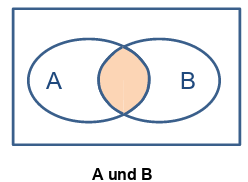
\includegraphics[width=.9\linewidth]{img/w06-wahrscheinlichkeit-and.png}
\end{center}
\begin{center}
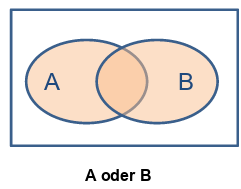
\includegraphics[width=.9\linewidth]{img/w06-wahrscheinlichkeit-or.png}
\end{center}
\begin{center}
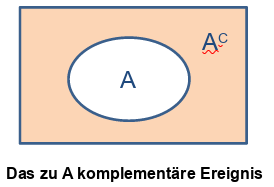
\includegraphics[width=.9\linewidth]{img/w06-wahrscheinlichkeit-not.png}
\end{center}
\begin{center}
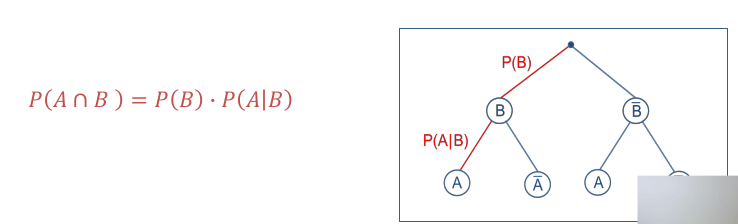
\includegraphics[width=.9\linewidth]{img/w06-wahrscheinlichkeit-bedingte.png}
\end{center}

\begin{itemize}
\item Laplace-Experiment
\item stochastisch unabhängig
\end{itemize}

\textbf{Wahrscheinlichkeitsmass-Regeln}:
\begin{equation*}
P(A \cup B) = P(A) + P(B) - P(A \cap B)
\end{equation*}
\begin{equation*}
P(A \cap B) = P(A) \cdot P(B)
\end{equation*}
\begin{align*}
P(A \cap B) &= P(B \cap A) \\
P(A) \cdot P(B|A) &= P(B) \cdot P(A|B)
\end{align*}
\begin{equation*}
P(A|B) = \frac{P(A \cap B)}{P(B)}
\end{equation*}

\textbf{Baysschen Regel}
\begin{equation*}
P(A) \cdot P(B|A) = P(B) \cdot P(A|B)
\end{equation*}

\textbf{Laplace-Experiment}
\begin{equation*}
P(A) = \frac{|A|}{|\Omega|}
\end{equation*}

\textbf{Vollständige Wahrscheinlichkeit}:
\begin{align*}
\bigcup_{i}^{n} B_i &= \Omega \text{ und } P(B_i) > 0 \forall i \\
P(A) &= \sum_{i}^{n} P(A|B_i) \cdot P(B_i) \\
&= \sum_{i}^{n} \frac{P(A \cap B) \cdot P(B)}{P(B)} \\
&= \sum_{i}^{n} P(A \cap B)
\end{align*}
\begin{center}
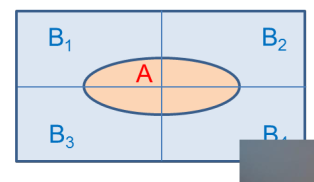
\includegraphics[width=.9\linewidth]{img/w07-wahrscheinlichkeit-vollstaendige-wahrscheinlichkeit.png}
\end{center}

\section*{Kombinatorik}
\label{sec:orgb48dea1}
\begin{itemize}
\item Mengen (Reihenfolge unwichtig)
\item Tupel (Reihenfolge \textbf{wichtig})
\item Urnenexperiment
\begin{itemize}
\item Kugel zurücklegen (wiederholen)
\item Reihenfolge beachten (geordnet)
\end{itemize}
\end{itemize}


\begin{itemize}
\item Geordnete Proben mit Wiederholung
\begin{itemize}
\item Pin Code iPhone (4 Stellen, 10 Ziffern entsprechen \(10^4\) Möglichkeiten)
\end{itemize}
\item Geordnete Proben ohne Wiederholung
\begin{itemize}
\item Anzahl Möglichkeiten: \(A = n (n-1) (n-2) ... (n-k+)\)
\item Formel: \(A = \frac{n!}{(n-k)!}\)
\end{itemize}
\end{itemize}

\textbf{Anzahl Permutation einer n-Menge}:
\begin{align*}
n!
\end{align*}

\textbf{Binominal Koeffizient}:
\begin{align*}
\binom{n}{k} = \frac{n(n-1)..(n-k+)}{k!}
\end{align*}

\textbf{Reihenfolge relevant, mit Zurücklegen}:
\begin{align*}
A = n^k
\end{align*}

\textbf{Reihenfolge nicht releveant, mit Zurücklegen}:
\begin{align*}
A = \binom{n+k-1}{k}
\end{align*}

\textbf{Reihenfolge relevant, ohne Zurücklegen}:
\begin{align*}
A &= \frac{n!}{(n-k)!} = \binom{n}{k} \cdot k!\\
A &= \prod_{n}^{(n-k+1)}n
\end{align*}

\textbf{Reihenfolge nicht relevant, ohne Zurücklegen}:
\begin{align*}
A = \frac{n!}{k!(n-k)!} = \binom{n}{k}
\end{align*}

\section*{Zufallsvariable und die wichtigsten theoretischen Verteilungen}
\label{sec:org535331f}
\begin{itemize}
\item Zufallsvariable, Abbildung / Funktion die den Elementen der Ergebnismenge eine Zahle zuordnet
\end{itemize}
\begin{align*}
X&: \{Wappen, Zahl\} \rightarrow \mathbb{R},  \\
X(\omega) &=
\begin{cases}
1, &  \quad \text{falls} \omega = \text{Wappen} \\
-1, & \quad \text{falls} \omega = \text{Zahl}
\end{cases}
\end{align*}

\begin{center}
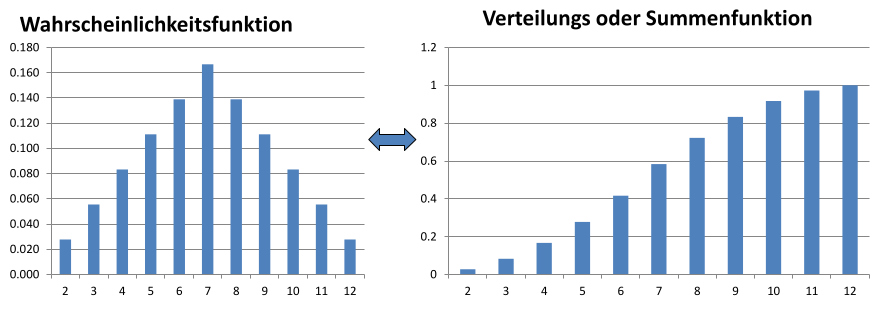
\includegraphics[width=.9\linewidth]{img/w08-wahrscheinlichkeitsfunktion-verteilsfunktion.png}
\end{center}

\subsubsection*{Diskrete Wahrscheinlichkeitsfunktion}
\label{sec:org1e39eb1}
\begin{itemize}
\item Summer aller Einzelwahrscheinlichkeit ist 1 (Fläche)
\end{itemize}
\begin{align*}
P(x_i \leq X \leq x_n) = \sum_{j=i}^{n} f(x_j)
\end{align*}

\begin{itemize}
\item Wichtige diskrete Verteilungen
\label{sec:orgef8a9e4}
\textbf{Bernoulli}:
\begin{itemize}
\item Binär (ja / nein)
\item Erfolgswahrscheinlichkeit \(p\) bleiben gleich
\end{itemize}
\begin{align*}
E(X) &= \overline{x} = p \\
\sigma^2 &= pq
\end{align*}

\textbf{Binominal}:
\begin{itemize}
\item Binär
\item wird n-mal wiederholt
\end{itemize}
\begin{equation*}
f(x) = \binom{n}{x}p^x(1-p)^{n-x}
\end{equation*}

\begin{equation*}
E(X) = np
\end{equation*}

\begin{equation*}
\sigma^2 = np(1-p)
\end{equation*}

\textbf{Poisonverteilung}:
\begin{itemize}
\item Näherung der Binominalverteilung wenn \(np \leq 10\) und \(n \geq 1500p\)
\item Wie hoch die Wahrscheinlichkeit, dass Ereignis E im Intervall I genau / höchstens x-mal auftritt, wenn bekannt ist, dass E \(\mu\) -mal auftritt
\item Anzahl Anrufe an der Hotline zwischen 10:00 und 12:00
\end{itemize}

\begin{equation*}
f(x) = P(X = x) = \frac{\mu^x}{x!}e^{-\mu}
\end{equation*}

\begin{equation*}
E(X) = \sigma^2 = \mu
\end{equation*}
\end{itemize}

\subsubsection*{Kontinuierliche Verteilungsdichtefunktion}
\label{sec:org3b0d2ae}
\begin{itemize}
\item Summer aller Wahrscheinlichkeit ist 1 (Fläche)
\item Die Berechnung der Wahrscheinlichkeit nur in Bereichen möglich
\end{itemize}

\begin{align*}
P(a \leq X \leq b) = \int_{a}^{b} f(x) dx
\end{align*}

\subsubsection*{Grundlegende Begriffe der Statistik}
\label{sec:org5346ee9}
\begin{itemize}
\item Erwartungs- oder Mittelwert: \(E[X] = \mu = \sum_{i} x_i f(x_i)\)
\end{itemize}
\section*{Stetige Verteilungen}
\label{sec:orga70de46}
\subsection*{Verteilungen}
\label{sec:org833734e}
\textbf{Normalverteilung}:
\begin{equation*}
z = \frac{x - \mu}{\sigma}
\end{equation*}

\textbf{Normalverteilung - Stichprobe}:
\begin{equation*}
Z_{stichprobe} = \frac{\overline{X} - \mu}{\frac{\sigma}{\sqrt{n}}}
\end{equation*}

\textbf{t-Verteilung}:
\begin{equation*}
t = \frac{\overline{x} - \mu}{\frac{\sigma}{\sqrt{n}}}
\end{equation*}

\begin{equation*}
r = n -1
\end{equation*}
\begin{equation*}
E(X) = 0 (\text{für} r > 1)
\end{equation*}

\begin{equation*}
\sigma^2 = \frac{r}{r-2} (\text{für} r > 2)
\end{equation*}

\textbf{Chi-Quadrat}:
\begin{equation*}
\chi_{(p,k)}^2
\end{equation*}

\begin{equation*}
E(X) = r
\end{equation*}
\begin{equation*}
\sigma^2 = 2r
\end{equation*}

Chi-Quadrat - untere Grenze:
\begin{equation*}
S_u = S \sqrt{\frac{n-1}{\chi_{(1-\frac{\alpha}{2},n-1)}^2}}
\end{equation*}

Chi-Quadrat - obere Grenze:
\begin{equation*}
S_o = S \sqrt{\frac{n-1}{\chi_{(\frac{\alpha}{2},n-1)}^2}}
\end{equation*}

\begin{itemize}
\item echte Zufallszahlen schlecht für Experimente
\item besser Pseudo-Zufallszahlen
\end{itemize}
\section*{{\bfseries\sffamily TODO} Schliessende Statistik}
\label{sec:org0f8d709}
\begin{enumerate}
\item Normalverteilung, wenn \(n \geq 30\)
\item t-Verteilung, wenn n \(n < 30\)
\item Chi Quadrat Verteilung
\end{enumerate}
\subsubsection*{Stichproben und Experimente}
\label{sec:orgd2e6b83}
\begin{enumerate}
\item Isolierende Abstraktion
\begin{itemize}
\item What are the objectives?
\end{itemize}
\item Generalisierende Abstraktion
\begin{itemize}
\item Modellverifikation
\item Modellvalidierung
\end{itemize}
\end{enumerate}
\subsubsection*{Chi-Quadrat-Verteilung}
\label{sec:orgb152577}
\begin{itemize}
\item Zufallsvariablen, die unabhängig und Normalverteilt sind:
\end{itemize}
\begin{equation*}
Y = X_1^2 + X_2^2 + X_3^2 + \cdots + X_r^2
\end{equation*}

\begin{center}
\begin{tabular}{ll}
"Echte" Grösse & Stichproben Grösse\\
\hline
\(\mu\) & \(\overline{X} \rightarrow \sigma_{\overline{x}}\)\\
\(\sigma\) & \(\hat{\sigma}\)\\
\end{tabular}
\end{center}

\begin{itemize}
\item Konfidenzintervall
\end{itemize}

\section*{{\bfseries\sffamily TODO} Schätzverfahren}
\label{sec:org0e67973}
\begin{itemize}
\item Nicht blind raten:
\begin{itemize}
\item Schätzverfahren
\item Schätzfunktionen
\item Gütekriterien für Schätzfunktionen
\end{itemize}

\item Schätzverfahren:
\begin{itemize}
\item die unbekannten Parameter anhand einer Stichprobe zu schätzen
\item durch Angabe eines Punktes: Punktschätzung
\item durch Angabe eines Intervalls: Intervallschätzung
\end{itemize}

\item Schätzfunktion:
\begin{itemize}
\item Punktschätzung: Hier werden die Werte für \(\mu\), \(\sigma^2\) und für unbekannte Wahrscheinlichkeiten p geschätzt
\item Intervallschätzung: Hier geht es um die Bestimmung eines Vertrauensintervall für die oben genannten Parametern
\end{itemize}
\end{itemize}

\subsubsection*{Erstellen eines Konfidenzintervall}
\label{sec:org62df8cd}
\begin{enumerate}
\item Feststellung der Verteilungsform von \(\overline{X}\) bzw. P
\item Festellung der Varianz von \(\overline{X}\) / P ggf. schätzen.
\item Ermittlung der Quantilwertes z oder t aus Tabelle / Rechner
\item Berechnung des maximalen Schätzfehlers (Produkt aus Quantilswert und Standardabweichung von X)
\item Ermittlung der Konfidenzgrenzen (Schätzfehler \(\pm\) Stichprobenmittel \(\overline{X}\)
\end{enumerate}

\section*{{\bfseries\sffamily TODO} Testverfahren}
\label{sec:org17e8b26}
\begin{itemize}
\item Testverfahren
\begin{itemize}
\item Parametertest
\item Verteilungs- bzw. Anpassungstest
\item Unabhängigkeitstest
\end{itemize}
\item Fehler
\begin{itemize}
\item Fehler erster Art (fehlerhaftes Ablehnen einer Hypothese)
\item Fehler zweiter Art (fehlerhaftes Annehmen einer Hypothese)
\end{itemize}
\end{itemize}


\begin{enumerate}
\item Fehler
\begin{itemize}
\item Wenn der ermittelte Werte ausserhalb des Annahmebereichs, wird die Hypothese verworfen
\end{itemize}
\item Fehler (siehe Bild)
\begin{itemize}
\item \(\mu1\) echter Wert, gemäss Hypothese ist H1 der Mittelwert
\item Nun wird die Hypothese angenommen; es wird ein Fehler gemacht
\end{itemize}
\begin{center}
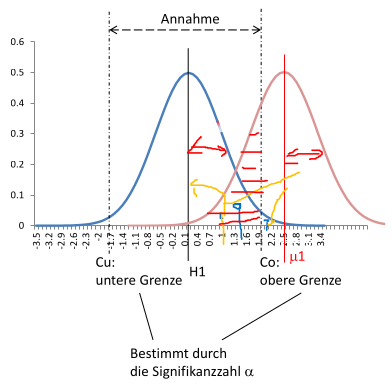
\includegraphics[width=.9\linewidth]{img/w12-testverfahren-2-fehler.png}
\end{center}
\end{enumerate}

\subsubsection*{Hypothese}
\label{sec:orge14218b}
\begin{enumerate}
\item Nullhypothese \(H_0\) und der Alternativhypothese \(H_1\) (im Allgemeinen die Verneinung der Nullhypothese)
\item Festlegen der Signifikanzzahl \(\alpha\), bzw. das Vertrauensintervall \(1-\alpha\)
\item Bestimmen der Testgrössen und Annahme- und Ablehungsbereiches
\item Berechnen der Werten
\end{enumerate}

Um die Hypothese zu beweisen, wird oft die Verneinung als Nullhypothese formuliert und versucht diese durch einen statistischen Test zu widerlegen.

\subsubsection*{Testverfahren}
\label{sec:org6179ad0}
\begin{itemize}
\item Parametertest
\item Anteilswert
\item Differenztests
\end{itemize}
\begin{itemize}
\item Abhängige Stichprobe
\label{sec:org3eb6f56}
\begin{enumerate}
\item Bilder der Nullhypothese \(H_0: \mu_1 = \mu_2\), folglich \(\overline{x} = 0\)
\item Die Differenzen der Stichprobe \(d_i = x_i - y_i\) für alle i erfassen
\item Die Nullhypothese \(H_0\) gilt, wenn der Mittelwert von \(d_i\) im Bereich von \(1-\alpha\) liegt
\item Signifikanzzahl \(\alpha\) wählen
\item Grenzen festlegen (mit Tabellen)
\end{enumerate}
\item Unabhängige Stichprobe
\label{sec:orgfffcce8}
\begin{enumerate}
\item Lege Signifikanzzahl \(\alpha\) fest
\item Mit Hilfe der Tabelle den Z-Wert festlegen
\item Berechne den Annahmebereich:
\begin{equation*}
  c = \pm z \sqrt{\frac{\sigma_1^2}{n_1}+\frac{\sigma_2^2}{n_2}}
\end{equation*}

\item Berechne die Mittelwerte der Stichproben \(\mu_1\) und \(\mu_2\)
\item Man nehme die Nullhypothese \(H_0: \mu_1 = \mu_2\) an, wenn die Differenz \(d_i = \mu_1 - \mu_2\) in den Annahmenbereich fällt
\end{enumerate}
\end{itemize}


\section*{TI-Nspire}
\label{sec:orgf440a9e}
\subsection*{Shortcuts}
\label{sec:org3c7e253}
Summenzeichen \(\Sigma\): \texttt{menu, 4, 5}

Produktzeichen \(\Pi\): \texttt{menu, 4, 6}

Fakultät !: \texttt{menu, 5, 1}

nCr: \texttt{menu, 5, 3}

solve: \texttt{menu, 3, 1}

Numerisch Lösen: \texttt{menu, 3, 6}

Ableitung: \texttt{menu, 4, 1}

Integral: \texttt{menu, 4, 3}

\subsection*{Funktionen}
\label{sec:org5d2951c}
Allgemein: \texttt{menu, 6, 3, <Zahl>}

Datensatzlänge: \texttt{count(x)}

Datensatzlänge mit Wert y: \texttt{count(x)}

Median: \texttt{median(x)}

Maximum: \texttt{max(x)}

Minimum: \texttt{min(x)}

Absoluter Wert: \texttt{abs(x)} oder \texttt{|x|}

Arithm. Mittelwert \(\overline{x}\): \texttt{mean(x)}

Empirishe-Varianz \(\sigma_x^2\): \texttt{varPop(x)}

Standardabweichung \(\sigma_x\): \texttt{stDevPop(x)}

Stichproben-Varianz: \texttt{varSamp(x)}

Summe \(\Sigma\): \texttt{sum(x)}

Approx. Zahlenwert \(\approx\): \texttt{approx(x)}

Kombinationen \(\binom{n}{k}\): \texttt{nCr(n,k)}

\subsection*{Verteilungen}
\label{sec:org8666d88}
Verteilungen die mit \emph{Pdf} (probability density function) enden sind die Dichtefunktionen f, solche die mit \emph{Cdf} (cumulative distribution function) enden sind die Verteilungsfunktionen F. Im Ti-Nspire zugänglich über \texttt{menu, 6, 5, <Zahl>}.


\subsubsection*{Normalverteilungs-}
\label{sec:org3045d69}

Dichte: \emph{normPdf(x, \(\mu\), \(\sigma\))}

Summe: \emph{normCdf(a, b, \(\mu\), \(\sigma\))}

Inverses: \emph{invNorm(\%, \(\mu\), \(\sigma\))}

z-Value: \emph{invNorm(\%, 0,1)}


\subsubsection*{Student-T Verteilungs-}
\label{sec:orgd7ad920}

Dichte: \texttt{tPdf(x, \textbackslash{}nu)}

Summe: \texttt{tCdf(a, b, \textbackslash{}nu)}

Inverses: \texttt{invT(\%, \textbackslash{}nu)}

\subsubsection*{\(\chi\)\textsuperscript{2}-Verteilungs-}
\label{sec:org58c633c}
Summe: \texttt{menu, 6, 5, 8, (a, b, \textbackslash{}nu)}

Inverse: \texttt{menu, 6, 5, 9, (\%, \textbackslash{}nu)}

\subsubsection*{Zentralle Konfidenzintervalle}
\label{sec:orga83b057}
\begin{enumerate}
\item \texttt{menu 6, 6, 1 (2 falls t)}
\item Dateneingabe: Statistik
\item \(\sigma\) = Standardabweichung (nicht Stichprobenwert)
\item \(\mu\) eintragen und \(n\) eintragen
\item Konfidenzniveau korrekt eintragen
\end{enumerate}

\subsection*{Liste}
\label{sec:orge2366d5}
Lineare Regression:
\begin{enumerate}
\item x-liste und y-liste eintragen
\item \texttt{menu, 6, 1, 4}
\end{enumerate}

Statistische Berechnungen:
\begin{enumerate}
\item x-liste (und y-liste) eintragen
\item \texttt{menu, 6, 1, <Zahl>}
\end{enumerate}

\subsection*{Spreadsheet}
\label{sec:org13a2508}
Datensatz hinzufügen:
\begin{enumerate}
\item Name in erste Zelle einfügen
\item Daten eintragen
\end{enumerate}


Spalte link einfügen: \texttt{menu, 2, 3}

Spalte verschieben: \texttt{menu, 1, 1}

Zellenname: SpalteIndex (e.g. a1)

Bereichsreferenz: Startzelle:Endzelle

Datensatz kopieren:
\begin{enumerate}
\item Shift + Pfeile (selektieren)
\item ctrl, c
\item Zu obersten Punkt neuer Spalte navigieren
\item ctrl, v
\end{enumerate}


Datensatz sortieren:
\begin{enumerate}
\item Spalte selektiren
\item \texttt{menu, 1, 6}
\end{enumerate}


Kumulierte Spalte hinzufügen:
\begin{enumerate}
\item In neuer Spalte ins Ausdruckszelle (Zweite Zellen von oben) gehen
\item \texttt{menu, 3, 7, 1} oder \texttt{cumultativeSum(<var>)}
\end{enumerate}


Gleitender Mittelwert:
\begin{enumerate}
\item Werte eintragen
\item In Zielspalte, Zelle \(n\) den Wert eintragen in der Form: (a1+a2+\ldots{}+an) / n
\item Mit selektierter Zelle: \texttt{menu, 3, 3}
\item Mit Pfeilen neue Zellen selektieren
\end{enumerate}


Newton-Alorithmus:
\begin{enumerate}
\item X-Werte in Spalte a, Y-Werte in Spalte b
\item In Zelle c2, den Wert \texttt{=approx((b2-b1)/(a2-a1))} eintragen
\item Mit selektierte Zelle: \texttt{menu, 3, 3}
\item Mit Pfeilen ganze Spalte ausfüllen
\item Ab Schritt 2 in Zelle d3 wiederholen: \texttt{=approx((c3-c2)/(a3-a1))}
\end{enumerate}



\newpage
\end{multicols}
\begin{multicols}{2}
\section*{Formelsammlung}
\label{sec:org6542903}
\subsection*{Lageparameter}
\label{sec:orgb04c5e0}
\begin{itemize}
\item \textbf{Klassenbreite}: \(b_m = x_m^o - x_m^u\)
\item \textbf{Klassenmitte}: \(\frac{x_m^o + x_m^u}{2}\)
\item \textbf{Klassendichte}: \(d_m = \frac{h_m}{b_j}\)
\end{itemize}

\textbf{Modus}:
Bei unterschiedlicher Klassenbreite anstellen von \(h_m\) Klassendichte nutzen.
\begin{equation*}
  Mo = x_m^u + \frac{h_m - h_{m-1}}{(h_m-h_{m-1})+(h_m-h_{m+1})}\cdot (x_m^o - x_m^u)
\end{equation*}

\textbf{Median}:
\begin{equation*}
  Me = x_m^u + \frac{\frac{n}{2}-H_{m-1}}{H_m - H_{m-1}} \cdot (x_m^o - x_m^u)
\end{equation*}
Quantile, Quartile, Dezile, Perzentile analog zu Median, einfach \(\frac{n}{2}\) passend ersetzen

\textbf{arithmetisches Mittel (mean, average)}:
\begin{align*}
\overline{x} &= \frac{1}{n} \sum_{i=1}^v x_i \cdot h_i \\
\overline{x} &= \frac{1}{n} \sum_{i=1}^v x_i \cdot f_i
\end{align*}

\textbf{arithmetisches Mittel - Klassifiziert} (\(\grave{x_i}\) Klassenmittelwert):
\begin{align*}
\overline{x} &= \frac{1}{n} \sum_{i=1}^v \grave{x_i} \cdot h_i \\
\overline{x} &= \frac{1}{n} \sum_{i=1}^v \grave{x_i} \cdot f_i
\end{align*}

\textbf{Harmonisches Mittel}:
Merkmal muss verhältnisskaliert sein
\begin{align*}
\overline{MH} = \frac{\sum_{i=1}^v h_i}{\sum_{i=1}^v \frac{h_i}{x_i}}
\end{align*}

\textbf{Geometrisches Mittel}:
\begin{align*}
MG = \sqrt[n]{\prod_{i=1}^n x_i} = \sqrt[n]{\frac{endwert}{anfangswert}}
\end{align*}

\textbf{Spannweite}:
\begin{equation*}
  R = x_{max} - x_{min}
\end{equation*}

\textbf{Zentraller Quartilsabstand}:
\begin{align*}
ZQA = Q_3 - Q_1
\end{align*}

\textbf{Mittlere absoulte Abweichung} (\(h_i\) absoulte Häufigkeit):
\begin{align*}
\delta = \frac{1}{n} \sum_{i=1}^{v}|x_i - \overline{x}| h_i
\end{align*}

\textbf{Varianz} (\(h_i\) absoulte Häufigkeit):
\begin{align*}
\sigma^2 &= \frac{1}{n} \sum_{i=1}^{v} (x_i - \overline{x})^2 h_i
\end{align*}

\textbf{Stichprobenvarianz} (\(h_i\) absoulte Häufigkeit):
\begin{align*}
  s^2 &= \frac{1}{n-1} \sum_{i=1}^{v} (x_i - \overline{x})^2 h_i \\
  &= \frac{n}{n-1}\sigma^2
\end{align*}

\begin{equation*}
\sigma_{\overline{x}}^2 = \frac{\sigma^2}{n}
\end{equation*}

\textbf{Standardabweichung} (Wurzerl der Varianz):
\begin{align*}
\sigma = \sqrt{\sigma^2} 
\end{align*}

\textbf{Variantionskoeffizienten}: Misst die relative Streuung
\begin{align*}
VK = \frac{\sigma}{\overline{x}} \cdot 100
\end{align*}

\textbf{Kovarianz}:
\begin{align*}
\sigma_{XY} &= \frac{1}{n}\sum_{i=1}^{n}(x_i-\overline{x})(y_i-\overline{y}) \\
\sigma_{XY} &= \frac{1}{n}\sum_{i=1}^{n}x_iy_i - \overline{x} \ \overline{y}
\end{align*}
Variante 2 Analog zu der Varianz

\textbf{Korrelationskoeffizient} (-1 - 1):
\begin{align*}
r &= \frac{\sigma_{XY}}{\sigma_X\sigma_Y} \quad mit \ |\sigma_{XY}| \leq \sigma_X\sigma_Y \\
r &= \frac{\sum_{i=1}^{n}(x_i-\overline{x})(y_i-\overline{y})}{\sqrt{(\sum_{i=1}^{n}(x_i-\overline{x})^2)(\sum_{i=1}^n(y_i-\overline{y})^2)}}
\end{align*}

\subsection*{Prognossen}
\label{sec:org65432de}
\textbf{gleitender Mittelwert}
\begin{align*}
M_t = \frac{1}{T+t}(\sum_{T=1}^{t-1} x_T +x_t)
\end{align*}

\textbf{Lineare Regression} funktioniert nur mit linearen zusammenhang. Bei einem exponentiellen kann dieser aber logrimiert werden. Bei einem logrimischen Zusammenhang kann potenziert werden um einen linearen Zusammenhang zu erhalten.
\begin{align*}
y &= a_1 + b_1x_i \\
a_1 &= \overline{y} - b_1\overline{x} \\
b_1 &= \frac{\sum_{i=1}^n x_iy_i - n\overline{x} \ \overline{y}}{\sum_{i=1}^n x_i^2 - n\overline{x}^2}
\end{align*}

\textbf{Newton - Algorithmus} (TI-Nspire):
\begin{align*}
f(x) = a_0 + a_1(x-x_1) + a_2(x-x_1)(x-x_2)+...+a_n(x-x_1)...(x-x_n)
\end{align*}
\subsection*{Anteilswert / Wahrscheinlichkeit (p)}
\label{sec:org59a5ac8}
k = Anzahl gute-Fälle, n = Stichprobenumfang
\begin{equation*}
\overline{p} = \frac{k}{n}
\end{equation*}

\subsection*{Fehler}
\label{sec:org582c5e6}
\textbf{Fehler}:
\begin{equation*}
e = z\frac{\sigma}{\sqrt{n}}
\end{equation*}
\textbf{Maximaler Fehler - mit zurücklegen (grosse Grundgesamtheit)}:
\begin{equation*}
n \geq \frac{z^2\sigma^2}{e^2}
\end{equation*}

\textbf{Maximaler Fehler - ohne zurücklegen}:
\begin{equation*}
n \geq \frac{z^2N\sigma^2}{e^2(N-1)+z^2\sigma^2}
\end{equation*}

\textbf{Vertrauensintervall - \(\overline{x}\)}:
\begin{equation*}
  \mu_0 - z \frac{\sigma}{\sqrt{n}} \leq \overline{x}\leq \mu_0 + z \frac{\sigma}{\sqrt{n}}
\end{equation*}

\textbf{Vertrauensintervall - Anteilswert}:
\begin{align*}
  c_u &= p_0 - z \sqrt{\frac{p_0(1-p0)}{n}} \\
  c_u &= p_0 - z \sqrt{\frac{p_0(1-p0)}{n}} \sqrt{\frac{N-n}{N-1}} \quad | \frac{n}{N} \geq 0.05
\end{align*}

\begin{align*}
  c_o &= p_0 + z \sqrt{\frac{p_0(1-p0)}{n}} \\
  c_o &= p_0 + z \sqrt{\frac{p_0(1-p0)}{n}} \sqrt{\frac{N-n}{N-1}} \quad | \frac{n}{N} \geq 0.05
\end{align*}

\end{multicols}

\subsection*{Varianz für das Stichprobenmittel \(\overline(X)\):}
\label{sec:orgaab308f}
\begin{center}
\begin{tabular}{lll}
Stichprobe & \(\sigma^2\) bekannt (\(\sigma_{\overline{X}}^2\)) & \(\sigma^2\) unbekannt (\(\hat{\sigma}_{\overline{X}}^2\))\\
\hline
Unendliche Grundgesamtheit & \(\frac{\sigma^2}{n}\) & \(\frac{s^2}{n}\)\\
\(\frac{n}{N} < 0.05\) & \(\approx \frac{\sigma^2}{n}\) & \(\approx \frac{s^2}{n}\)\\
\(\frac{n}{N} \geq 0.05\) & \(\frac{\sigma^2}{n} \cdot \frac{N-n}{N-1}\) & \(\frac{s^2}{n} \cdot \frac{N-n}{N}\)\\
\end{tabular}
\end{center}

\subsection*{Varianz für den Anteilswert (P):}
\label{sec:org7cea2af}

für \(np (1-P) > 9\) aprox. normalverteilt
\begin{center}
\begin{tabular}{lll}
Stichprobe & \(\sigma^2\) bekannt (\(\sigma_{P}^2\)) & \(\sigma^2\) unbekannt (\(\hat{\sigma}_{P}^2\))\\
\hline
Unendliche Grundgesamtheit & \(\frac{P(1-P)}{n}\) & \(\frac{P(1-P)}{n}\)\\
\(\frac{n}{N} < 0.05\) & \(\approx \frac{P(1-P)}{n}\) & \(\approx \frac{P(1-P)}{n}\)\\
\(\frac{n}{N} \geq 0.05\) & \(\frac{P(1-P)}{n} \cdot \frac{N-n}{N-1}\) & \(\frac{P(1-p)}{n} \cdot \frac{N-n}{N}\)\\
\end{tabular}
\end{center}
\end{document}